\documentclass[a4paper, 14pt]{extarticle}

% Поля
%--------------------------------------
\usepackage{geometry}
\geometry{a4paper,tmargin=2cm,bmargin=2cm,lmargin=3cm,rmargin=1cm}
%--------------------------------------

%Russian-specific packages
%--------------------------------------
\usepackage[T2A]{fontenc}
\usepackage[utf8]{inputenc}
\usepackage[english, main=russian]{babel}
%--------------------------------------

\usepackage{textcomp}

% Красная строка
%--------------------------------------
\usepackage{indentfirst}
%--------------------------------------

%Graphics
%--------------------------------------
\usepackage{graphicx}
\graphicspath{ {./images/} }
\usepackage{wrapfig}
%--------------------------------------

% Полуторный интервал
%--------------------------------------
\linespread{1.3}
%--------------------------------------

%Выравнивание и переносы
%--------------------------------------
\sloppy
\clubpenalty=10000
\widowpenalty=10000
%--------------------------------------

%Списки
\usepackage{enumitem}

%Подписи
\usepackage{caption}

%Гиперссылки
\usepackage{hyperref}
\hypersetup {
	unicode=true
}

%Rисунки
%--------------------------------------
\DeclareCaptionLabelSeparator*{emdash}{~--- }
\captionsetup[figure]{labelsep=emdash,font=onehalfspacing,position=bottom}
%--------------------------------------

\usepackage{tempora}
\usepackage{amsmath}
\usepackage{color}
\usepackage{listings}
\lstset{
  belowcaptionskip=1\baselineskip,
  breaklines=true,
  frame=L,
  xleftmargin=\parindent,
  language=C++,
  showstringspaces=false,
  basicstyle=\footnotesize\ttfamily,
  keywordstyle=\bfseries\color{blue},
  commentstyle=\itshape\color{purple},
  identifierstyle=\color{black},
  stringstyle=\color{red},
}

%--------------------------------------
%			НАЧАЛО ДОКУМЕНТА
%--------------------------------------

\begin{document}

%--------------------------------------
%			ТИТУЛЬНЫЙ ЛИСТ
%--------------------------------------
\begin{titlepage}
\thispagestyle{empty}
\newpage

%Шапка титульного листа
%--------------------------------------
\vspace*{-60pt}
\hspace{-65pt}
\begin{minipage}{0.3\textwidth}
\hspace*{-20pt}\centering

\includegraphics[width=\textwidth]{emblem}
\end{minipage}
\begin{minipage}{0.67\textwidth}\small \textbf{
\vspace*{-0.7ex}
\hspace*{-6pt}\centerline{Министерство науки и высшего образования Российской Федерации}
\vspace*{-0.7ex}
\centerline{Федеральное государственное бюджетное образовательное учреждение }
\vspace*{-0.7ex}
\centerline{высшего образования}
\vspace*{-0.7ex}
\centerline{<<Московский государственный технический университет}
\vspace*{-0.7ex}
\centerline{имени Н.Э. Баумана}
\vspace*{-0.7ex}
\centerline{(национальный исследовательский университет)>>}
\vspace*{-0.7ex}
\centerline{(МГТУ им. Н.Э. Баумана)}}
\end{minipage}
%--------------------------------------

%Полосы
%--------------------------------------
\vspace{-25pt}
\hspace{-35pt}\rule{\textwidth}{2.3pt}

\vspace*{-20.3pt}
\hspace{-35pt}\rule{\textwidth}{0.4pt}
%--------------------------------------

\vspace{1.5ex}
\hspace{-35pt} \noindent \small ФАКУЛЬТЕТ\hspace{80pt} <<Информатика и системы управления>>

\vspace*{-16pt}
\hspace{47pt}\rule{0.83\textwidth}{0.4pt}

\vspace{0.5ex}
\hspace{-35pt} \noindent \small КАФЕДРА\hspace{50pt} <<Прикладная Математика и информатика>>

\vspace*{-16pt}
\hspace{30pt}\rule{0.866\textwidth}{0.4pt}

\vspace{11em}

\begin{center}
\Large {\bf Лабораторная работа № 7} \\
\large {\bf по курсу <<Языки и методы программирования>>} \\
\large {\bf <<Разработка простейшего класса на C++>>}
\end{center}\normalsize

\vspace{8em}

\begin{flushright}
  {Студент группы ИУ9-21Б Хромов М.\,А.\hspace*{15pt} \\
  \vspace{2ex}
  Преподаватель Посевин Д.\,П.\hspace*{15pt}}
\end{flushright}

\bigskip

\vfill

\begin{center}
\textsl{Москва 2025}
\end{center}
\end{titlepage}
%--------------------------------------
%		КОНЕЦ ТИТУЛЬНОГО ЛИСТА
%--------------------------------------

\renewcommand{\ttdefault}{pcr}
\setlength{\tabcolsep}{3pt}
\newpage

%--------------------------------------
\section{Задание}\label{Sect::task}
%--------------------------------------
Выполнение лабораторной работы заключается в составлении на языке C++ программы, состоящей из трёх файлов:
\begin{itemize}[nosep]
    \item заголовочный файл \texttt{declaration.h} с объявлением одного из классов, приведённых в таблицах 1~--~16;
    \item файл \texttt{implementation.cpp} с определениями методов класса;
    \item файл \texttt{main.cpp}, содержащий функцию \texttt{main} и, при необходимости, вспомогательные функции для проверки работоспособности класса.
\end{itemize}

Реализация класса \textbf{не должна} опираться на стандартные контейнерные классы C++, то есть внутреннее состояние объектов должно быть реализовано через обычные динамические массивы. В классе обязательно требуется реализовать:
\begin{itemize}[nosep]
    \item конструктор копий;
    \item виртуальный деструктор;
    \item операцию присваивания.
\end{itemize}

Проверку работоспособности необходимо организовать в \texttt{main.cpp} и включить:
\begin{enumerate}[nosep]
    \item создание объекта класса в автоматической памяти;
    \item передачу объекта класса по значению в функцию;
    \item присваивание объекта класса другой переменной.
\end{enumerate}

%--------------------------------------
\section{Индивидуальный вариант}\label{Sect::variant}
%--------------------------------------

\subsection*{Вариант 22}
\textbf{Последовательность символов ASCII} с поддержкой операций:
\begin{enumerate}[nosep]
    \item получение количества символов;
    \item получение ссылки на $i$-тый символ;
    \item вставка нового символа в $i$-тую позицию;
    \item проверка, является ли последовательность палиндромом.
\end{enumerate}

\subsection*{Вариант 23}
\textbf{Беззнаковое рациональное число}, представленное в позиционной системе счисления по основанию $d$, часть цифр которого может быть неизвестна. Число задаётся вектором цифр ( каждое целое от $0$ до $d-1$) и позицией точки, разделяющей целую и дробную части.

Цифры целой части нумеруются неотрицательными числами (младшая~--~$0$), цифры дробной части~--~отрицательными (старшая~--~$-1$). Позиция точки может быть отрицательной или превышать количество цифр.

Операции класса:
\begin{enumerate}[nosep]
    \item получение количества цифр;
    \item определение, известна ли $i$-тая цифра (за пределами диапазона считать известной и равной~$0$);
    \item получение ссылки на $i$-тую цифру с автоматическим расширением и возможностью «обнулить» ранее неизвестную цифру;
    \item округление числа до указанного количества значащих цифр.
\end{enumerate}

Конструктор принимает основание $d$, количество цифр $n$ и позицию точки $p$ и порождает число, все цифры которого неизвестны.

%--------------------------------------
\section{Практическая реализация}
%--------------------------------------

\subsection*{Листинг 1. \texttt{main.cpp} для варианта 22}
\begin{figure}[!htb]
\begin{lstlisting}[language=C++,caption={main.cpp для ASCIISequence},label={lst:code1}]
#include <iostream>
#include "declaration.h"

using namespace std;

void testASCIISequence(ASCIISequence seq) {
    cout << "1. Количество символов: " << seq.getSize() << endl;

    try {
        cout << "2. Символ на позиции 1: " << seq.getChar(1) << endl;
    } catch (const out_of_range& e) {
        cout << "Ошибка: " << e.what() << endl;
    }
}

int main() {
    ASCIISequence seq1;
    cout << "Создаём последовательность...\n";

    seq1.insertChar(0, 'a');
    seq1.insertChar(1, 'b');
    seq1.insertChar(2, 'c');

    cout << "После вставки 'a', 'b', 'c': ";
    for (size_t i = 0; i < seq1.getSize(); ++i)
        cout << seq1.getChar(i);
    cout << endl;

    cout << "Палиндром? " << (seq1.isPalindrome() ? "Да" : "Нет") << endl;

    testASCIISequence(seq1);

    ASCIISequence seq2;
    seq2 = seq1;
    cout << "После присваивания seq2 = seq1: ";
    for (size_t i = 0; i < seq2.getSize(); ++i)
        cout << seq2.getChar(i);
    cout << endl;

    seq1.insertChar(1, 'z');
    cout << "После вставки 'z' на позицию 1: ";
    for (size_t i = 0; i < seq1.getSize(); ++i)
        cout << seq1.getChar(i);
    cout << endl;

    cout << "Палиндром после вставки 'z'? "
         << (seq1.isPalindrome() ? "Да" : "Нет") << endl;
    return 0;
}
\end{lstlisting}
\end{figure}

\subsection*{Листинг 2. \texttt{implementation.cpp} для ASCIISequence}
\begin{figure}[!htb]
\begin{lstlisting}[language=C++,caption={implementation.cpp для ASCIISequence},label={lst:code2}]
#include "declaration.h"
#include <cstring>
#include <stdexcept>

ASCIISequence::ASCIISequence() : sequence(nullptr), size(0) {}

ASCIISequence::ASCIISequence(const ASCIISequence& other) : size(other.size) {
    sequence = new char[size];
    std::memcpy(sequence, other.sequence, size);
}

ASCIISequence& ASCIISequence::operator=(const ASCIISequence& other) {
    if (this == &other) return *this;
    delete[] sequence;
    size = other.size;
    sequence = new char[size];
    std::memcpy(sequence, other.sequence, size);
    return *this;
}

ASCIISequence::~ASCIISequence() {
    delete[] sequence;
}

size_t ASCIISequence::getSize() const {
    return size;
}

char& ASCIISequence::getChar(size_t index) {
    if (index >= size)
        throw std::out_of_range("index out of range");
    return sequence[index];
}

void ASCIISequence::insertChar(size_t index, char c) {
    if (index > size)
        throw std::out_of_range("index out of range");

    char* newSeq = new char[size + 1];
    std::memcpy(newSeq, sequence, index);
    newSeq[index] = c;
    std::memcpy(newSeq + index + 1, sequence + index, size - index);

    delete[] sequence;
    sequence = newSeq;
    ++size;
}

bool ASCIISequence::isPalindrome() const {
    for (size_t i = 0; i < size / 2; ++i)
        if (sequence[i] != sequence[size - i - 1])
            return false;
    return true;
}
\end{lstlisting}
\end{figure}

\subsection*{Листинг 3. \texttt{declaration.h} для ASCIISequence}
\begin{figure}[!htb]
\begin{lstlisting}[language=C++,caption={declaration.h для ASCIISequence},label={lst:code3}]
#pragma once
#include <cstddef>

class ASCIISequence {
private:
    char*  sequence;
    size_t size;

public:
    ASCIISequence();
    ASCIISequence(const ASCIISequence& other);
    ASCIISequence& operator=(const ASCIISequence& other);
    virtual ~ASCIISequence();

    size_t getSize() const;
    char&  getChar(size_t index);
    void   insertChar(size_t index, char c);
    bool   isPalindrome() const;
};
\end{lstlisting}
\end{figure}

\subsection*{Листинг 4. \texttt{main.cpp} для варианта 23}
\begin{figure}[!htb]
\begin{lstlisting}[language=C++,caption={main.cpp для RationalNumber},label={lst:code4}]
#include <iostream>
#include "declaration.h"

using namespace std;

void testFunction(RationalNumber num) {
    cout << "Тест передачи по значению. Длина: " << num.length() << endl;
}

int main() {
    RationalNumber num(10, 5, 2);
    cout << "Начальная длина: " << num.length() << endl;

    num.digit(0)  = 7;
    num.digit(1)  = 3;
    num.digit(-1) = 9;

    cout << "Число: " << num.toString(-2, 2) << endl;
    cout << "Известна цифра 0? "  << num.isKnown(0)  << endl;
    cout << "Известна цифра 2? "  << num.isKnown(2)  << endl;
    cout << "Известна цифра -7? " << num.isKnown(-7) << endl;

    cout << "Цифра 0: "  << num.digit(0)  << endl;
    cout << "Цифра -1: " << num.digit(-1) << endl;
    cout << "Цифра 2: "  << num.digit(2)  << endl;

    cout << "Известна цифра -3 после обращения? "
         << num.isKnown(-3) << endl;

    cout << "Длина после обращения к -3: "
         << num.length() << endl;

    testFunction(num);

    RationalNumber another(10, 3, 1);
    another = num;
    cout << "После присваивания another = num, цифра 0: "
         << another.digit(0) << endl;
    return 0;
}
\end{lstlisting}
\end{figure}

\subsection*{Листинг 5. \texttt{declaration.h} для RationalNumber}
\begin{figure}[!htb]
\begin{lstlisting}[language=C++,caption={declaration.h для RationalNumber},label={lst:code5}]
#pragma once
#include <string>

class RationalNumber {
    int  base;
    int  size;
    int  pointPos;
    int* digits;
    bool* known;

public:
    RationalNumber(int d, int n, int p);
    RationalNumber(const RationalNumber& other);
    RationalNumber& operator=(const RationalNumber& other);
    virtual ~RationalNumber();

    int  length() const;
    bool isKnown(int i) const;
    int& digit(int i);
    void round(int significantDigits);
    std::string toString(int from, int to) const;

private:
    void resize(int newIndex);
};
\end{lstlisting}
\end{figure}

\subsection*{Листинг 6. \texttt{implementation.cpp} для RationalNumber}
\begin{figure}[!htb]
\begin{lstlisting}[language=C++,caption={implementation.cpp для RationalNumber},label={lst:code6}]
#include "declaration.h"
#include <cstring>
#include <sstream>
#include <stdexcept>

using namespace std;

RationalNumber::RationalNumber(int d, int n, int p)
    : base(d), size(n), pointPos(p) {
    digits = new int[size];
    known  = new bool[size];
    for (int i = 0; i < size; ++i) {
        digits[i] = 0;
        known[i]  = false;
    }
}

RationalNumber::RationalNumber(const RationalNumber& other)
    : base(other.base), size(other.size), pointPos(other.pointPos) {
    digits = new int[size];
    known  = new bool[size];
    memcpy(digits, other.digits, sizeof(int)  * size);
    memcpy(known,  other.known,  sizeof(bool) * size);
}

RationalNumber& RationalNumber::operator=(const RationalNumber& other) {
    if (this == &other) return *this;
    delete[] digits;
    delete[] known;

    base      = other.base;
    size      = other.size;
    pointPos  = other.pointPos;
    digits    = new int[size];
    known     = new bool[size];
    memcpy(digits, other.digits, sizeof(int)  * size);
    memcpy(known,  other.known,  sizeof(bool) * size);
    return *this;
}

RationalNumber::~RationalNumber() {
    delete[] digits;
    delete[] known;
}

int RationalNumber::length() const { return size; }

bool RationalNumber::isKnown(int i) const {
    int idx = pointPos - i - 1;
    if (idx < 0 || idx >= size) return true;
    return known[idx];
}

void RationalNumber::resize(int newIdx) {
    if (newIdx < size) return;
    int newSize = newIdx + 1;
    int*  newDigits = new int[newSize];
    bool* newKnown  = new bool[newSize];

    for (int i = 0; i < newSize; ++i) {
        if (i < size) {
            newDigits[i] = digits[i];
            newKnown[i]  = known[i];
        } else {
            newDigits[i] = 0;
            newKnown[i]  = false;
        }
    }
    delete[] digits;
    delete[] known;
    digits = newDigits;
    known  = newKnown;
    size   = newSize;
}

int& RationalNumber::digit(int i) {
    int idx = pointPos - i - 1;

    if (idx < 0) {                // расширение в старший разряд
        int shift = -idx;
        int newSize = size + shift;
        int*  newDigits = new int[newSize];
        bool* newKnown  = new bool[newSize];

        for (int j = 0; j < shift; ++j) {
            newDigits[j] = 0; newKnown[j] = false;
        }
        for (int j = 0; j < size; ++j) {
            newDigits[j + shift] = digits[j];
            newKnown [j + shift] = known [j];
        }
        delete[] digits;
        delete[] known;
        digits   = newDigits;
        known    = newKnown;
        pointPos += shift;
        size     = newSize;
        idx      = 0;
    } else if (idx >= size) {
        resize(idx);
    }

    if (!known[idx]) {
        known[idx]  = true;
        digits[idx] = 0;
    }
    return digits[idx];
}

string RationalNumber::toString(int from, int to) const {
    ostringstream oss;
    for (int i = to; i >= from; --i) {
        if (i == 0) oss << '.';
        int idx = pointPos - i - 1;
        if (idx < 0 || idx >= size || !known[idx])
            oss << '?';
        else
            oss << digits[idx];
    }
    return oss.str();
}

void RationalNumber::round(int significantDigits) {
    // Простая демонстрационная реализация (округление вниз).
    // Реализовать более точную логику при необходимости.
    int target = significantDigits - 1 - pointPos;
    if (target < 0) return;
    if (target >= size) return;
    for (int i = 0; i < target; ++i) {
        known[i]  = true;
        digits[i] = 0;
    }
}
\end{lstlisting}
\end{figure}
\clearpage
\newpage
%--------------------------------------
\section{Реализация}
%--------------------------------------
\begin{center}
    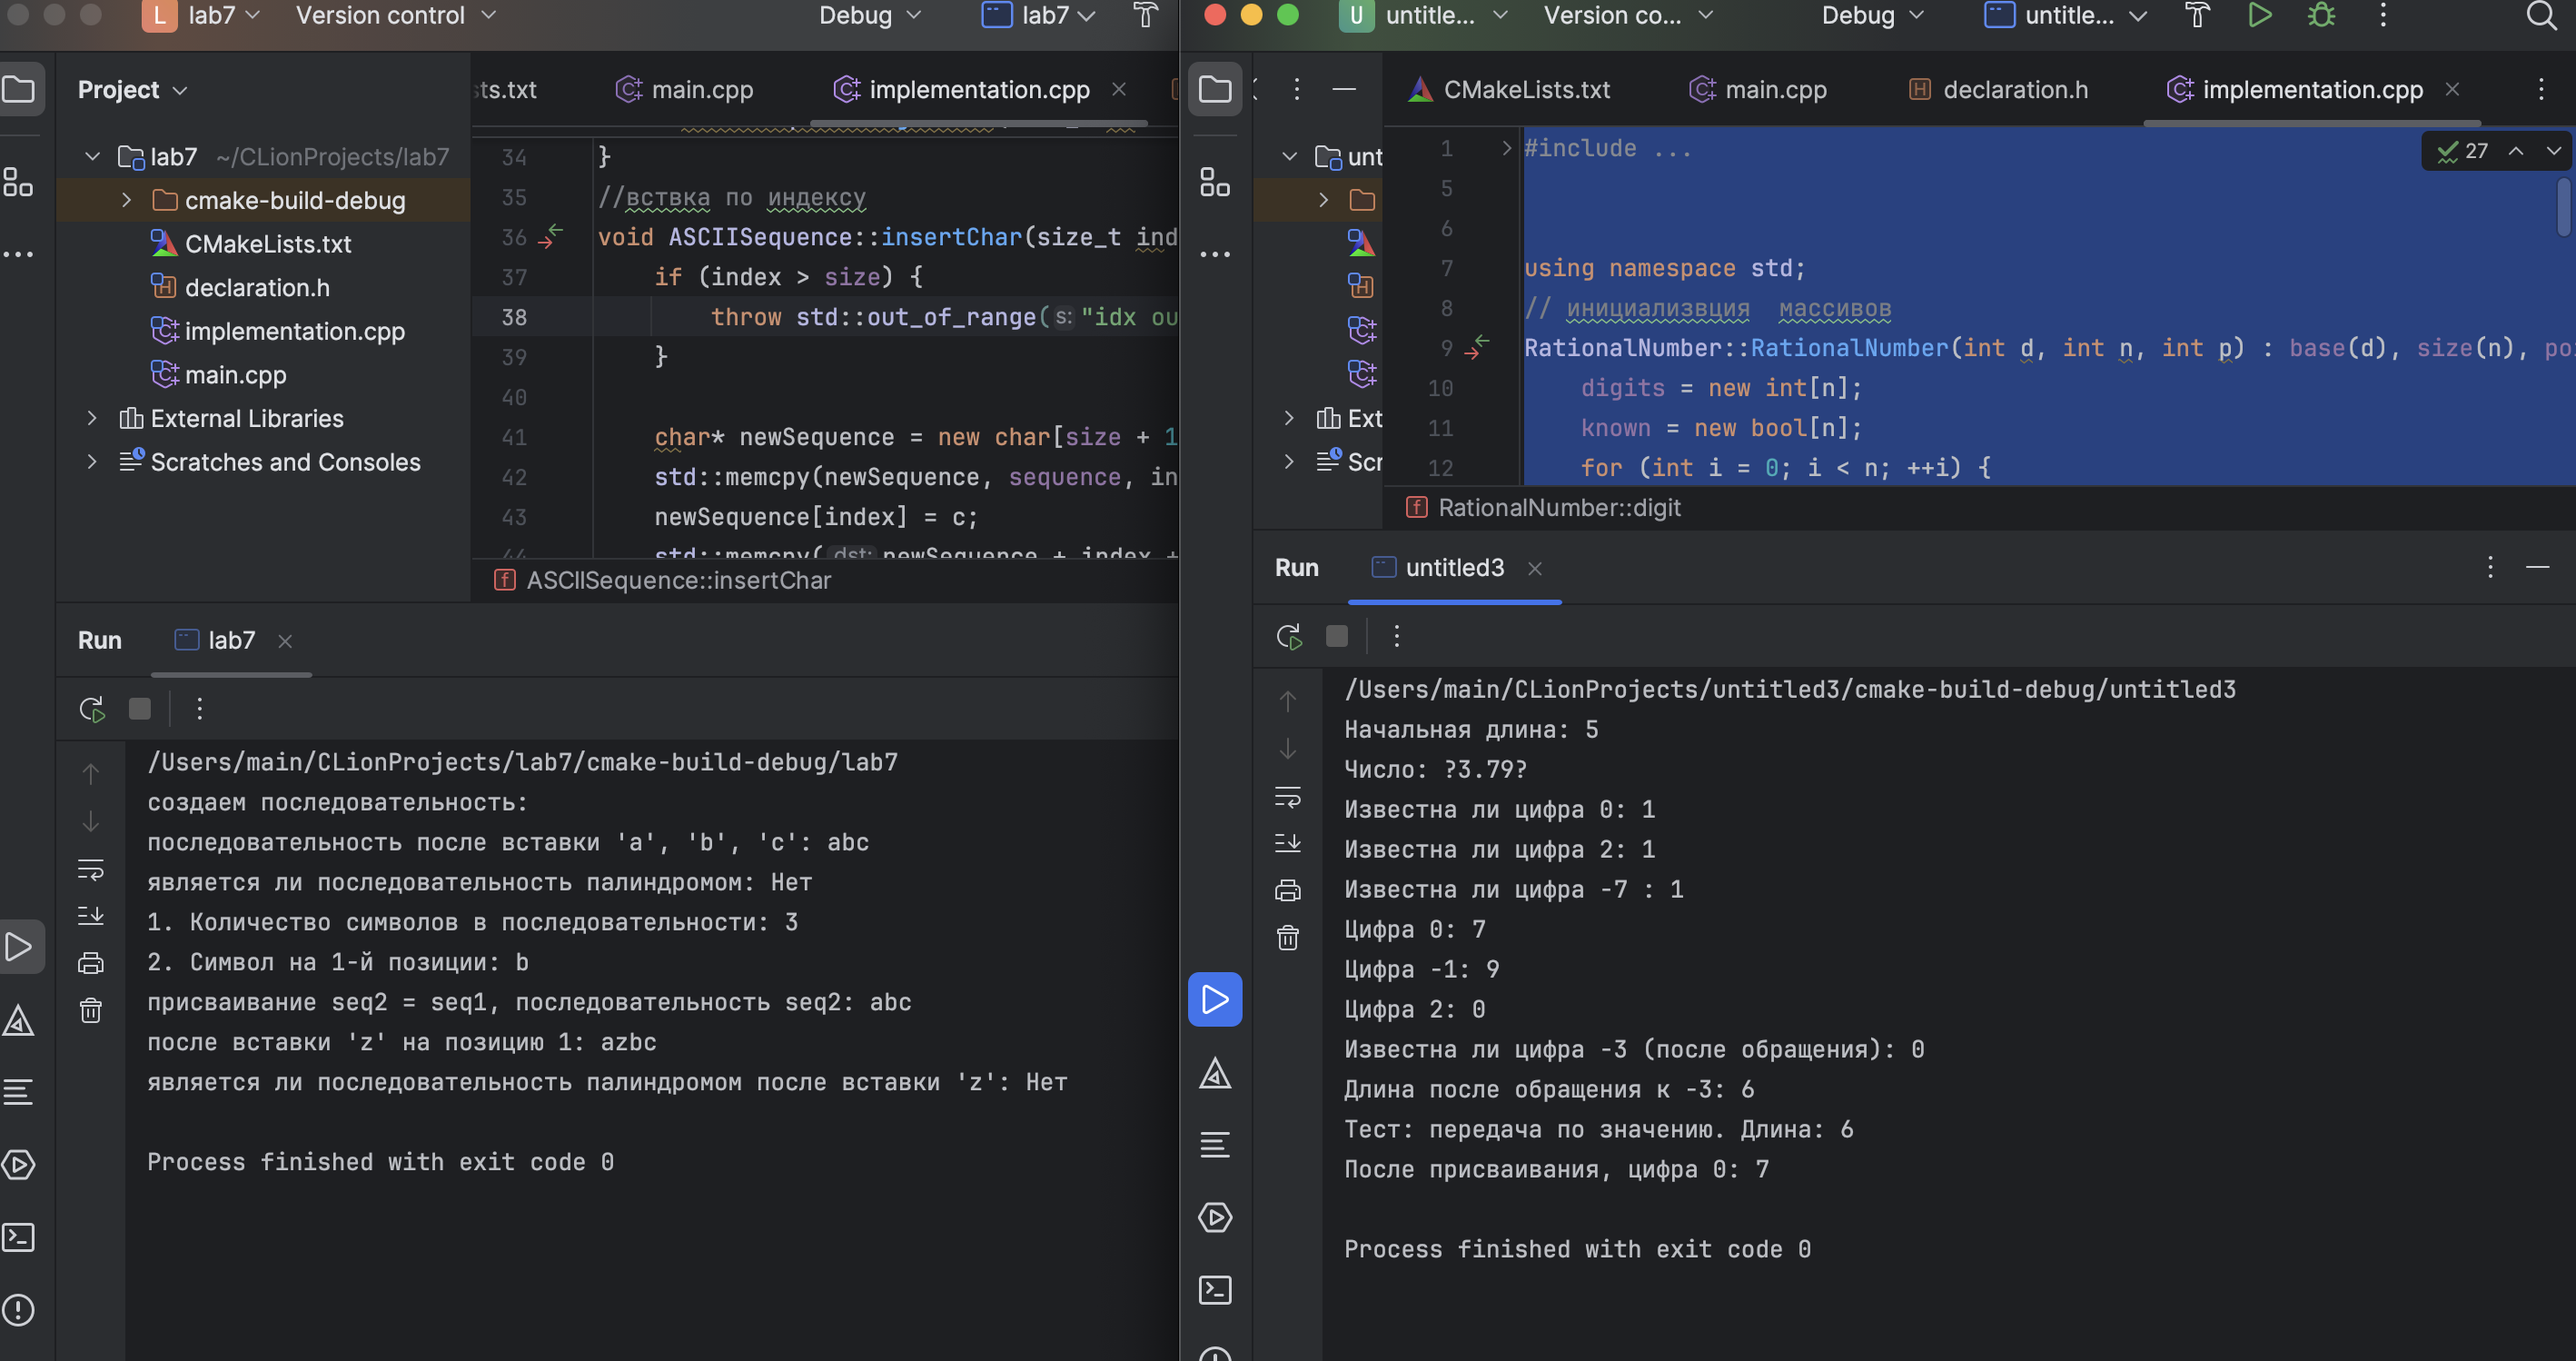
\includegraphics[width=0.8\textwidth]{фото19.jpeg}
    \captionof{figure}{вывод программы}
\end{center}
\newpage
%--------------------------------------
\section{Вывод}
%--------------------------------------
В лабораторной работе были разработаны два пользовательских контейнерных класса\,---\,\texttt{ASCIISequence} и \texttt{RationalNumber}:

\begin{itemize}[nosep]
    \item Реализованы динамические массивы собственного управления без использования стандартных контейнеров STL.
    \item Для каждого класса обеспечены \textbf{правило трёх}: конструктор копии, виртуальный деструктор и оператор присваивания.
    \item Разработаны функции проверки: передача объектов по значению, присваивание и базовый набор операций по условию варианта.
    \item Для \texttt{ASCIISequence} продемонстрированы операции вставки символов, подсчёта длины и проверки палиндрома.
    \item Для \texttt{RationalNumber} реализованы операции доступа к цифрам в произвольной позиции и текстового вывода числа с неизвестными цифрами.
\end{itemize}

В результате получены полностью работоспособные классы, иллюстрирующие принципы управления памятью в C++ и применение объектно-ориентированного подхода к построению абстрактных типов данных.
\end{document}
